\documentclass[UTF8,ctexart,a4paper,11pt,openany]{article}
\usepackage[slantfont,boldfont]{xeCJK}
\usepackage{fontspec}
\usepackage{ctex}
\usepackage{algpseudocode}
\setCJKmainfont{SimSun}%[BoldFont=SimHei] %去掉注释:bf字体为黑体

\setsansfont{SimHei}
\setCJKsansfont{SimHei}

\xeCJKsetcharclass{"2160}{"2470}{1}% 1: CJK
\xeCJKsetup{AutoFallBack=true}
\setCJKfallbackfamilyfont{\CJKrmdefault}{SimSun.ttf}

%\setmainfont{Times New Roman}     %去掉注释:Times new roman字体
%\usepackage{mathptmx}             %去掉注释:Times new roman字体

\usepackage{mathtools}
\usepackage{amsmath}
\usepackage{amsfonts}
\usepackage{amssymb}
\usepackage{amsthm}
\usepackage[T1]{fontenc}
\usepackage{indentfirst} %段首空两格

\usepackage{graphicx}
\usepackage{geometry}
\usepackage{latexsym}
\usepackage{fancyhdr}
\usepackage{epstopdf}
%\usepackage{pifont}
%\usepackage[perpage,symbol*]{footmisc}
\usepackage{titlesec}
\usepackage{setspace}
\usepackage{enumerate}
\usepackage{enumitem}
\usepackage{multicol}
\usepackage{url}
\usepackage{exscale}
\usepackage{ulem}
\usepackage{relsize}
\usepackage{mathrsfs}
\usepackage{tikz}
\usepackage{wrapfig}
\usepackage{framed}
\usepackage{bm}
%\usepackage{pstricks,pst-node,multido,ifthen,calc}
\usepackage[all]{xy}
\usepackage{extarrows}
%\usepackage[backref]{hyperref}
\usepackage{hyperref}
\usepackage{stfloats} %插图的时候不分页

\setlength{\parindent}{2em} %段首空两格
\linespread{1.2}
\usepackage{listings}
\usepackage{xcolor}
\usepackage{algorithm}
\usepackage{algorithmicx}
\usepackage{algpseudocode}
\usepackage{mdframed}
\usepackage{extarrows}
\usepackage{diagbox}
\usepackage{makecell}

\theoremstyle{definition}
\mdfdefinestyle{theoremstyle}{%
linecolor=green!40,linewidth=.5pt,%
backgroundcolor=green!10,
skipabove=8pt,
skipbelow=5pt,
innerleftmargin=7pt,
innerrightmargin=7pt,
frametitlerule=true,%
frametitlerulewidth=.5pt,
frametitlebackgroundcolor=green!35,
frametitleaboveskip=0pt,
frametitlebelowskip=0pt,
innertopmargin=.4\baselineskip,
innerbottommargin=.4\baselineskip,
shadow=true,shadowsize=3pt,shadowcolor=black!20,
%theoremseparator={\hspace{1pt}},
theoremseparator={.},
nobreak=true,
}


\everymath{\displaystyle}

\newtheorem{definition}{\hspace{2em}定义}[section]
\newtheorem{axiom}{\hspace{2em}公理}

\mdtheorem[style=theoremstyle]{theorem}{定理}
\mdtheorem[style=theoremstyle]{example}{例}
\mdtheorem[style=theoremstyle]{exercise}{问题}
\newtheorem{lemma}[theorem]{\hspace{2em}引理}
\newtheorem{corollary}[theorem]{\hspace{2em}推论}

\newcommand*{\QED}{\hfill\ensuremath{\square}}
\newcommand*{\rmk}{\textbf{注:}}
\renewcommand*{\proof}{\textbf{证明:}}
\newcommand*{\tips}{\textbf{提示:}}
\newcommand*{\hard}{\textbf{\color{red}(难)}}
\newcommand*{\eqsmall}{\setlength\abovedisplayskip{1pt}\setlength\belowdisplayskip{1pt}}
\geometry{left=2cm,right=2cm,top=2cm,bottom=2cm}
% \title{数值分析上机报告(示例}
% \author{Fiddie}
\pagestyle{fancy}
\fancyfoot[C]{}
\fancyhead[RO]{ \thepage}
\fancyhead[LE]{\thepage  }
% \fancyhead[RE]{\rightmark (By Fiddie)}
% \fancyhead[LO]{\leftmark (By Fiddie)}
\titleformat{\chapter}{\centering\huge\bfseries}{第\,\thechapter\,章}{1em}{} %更改标题样式
\titleformat{\section}{\bfseries\Large}{$\S$\,\thesection\,}{1em}{} %更改标题样式
\titlespacing*{\chapter}{0pt}{9pt}{0pt} %调整标题间距
\setenumerate[1]{itemsep=0pt,partopsep=0pt,parsep=\parskip,topsep=0pt} %设置enumerate行间距
\setenumerate[2]{itemsep=0pt,partopsep=0pt,parsep=\parskip,topsep=0pt} %设置enumerate行间距
\setitemize[1]{itemsep=0pt,partopsep=0pt,parsep=\parskip,topsep=0pt} % 设置itemize行间距
\setlist[enumerate,2]{label=(\arabic*),topsep=0mm,itemsep=0mm,partopsep=0mm,parsep=\parskip}
    % 设置二层枚举为(1)样式
    
\newfontfamily\hei{SimHei}
\newcommand\textcf[1]{\textbf{\textsf{\hei{#1}}}}

\newcommand\e{\leftarrow}
%\renewcommand{\bibname}{参考文献}

\begin{document}
\begin{center}
{\huge \textbf{数值分析第6次上机作业}}

{\large 学号:221840189,姓名:王晨光}
\end{center}

\section{问题}
实现快速傅里叶变换FFT,并应用于某个具体场景。如信号,图像,声音处理,多项式乘法,偏微分方程求解(谱方法),或其它应用场景。
\section{算法思路}
\subsection{快速傅里叶变换(FFT)}
FFT快速傅里叶变换算法利用了复数单位根的性质极大了提高了离散傅里叶变换算法的效率,将原本$O(n^2)$的时间复杂度降低到了$O(n\log{n})$。\\
\par DFT的计算可归结为计算
\[
    c_k=\sum_{j=0}^{N-1}x_j w^{k j} (k=0,1,\cdots,N-1)
\]
其中$w=e^{-\mathrm{i}\frac{2\pi}{N}}$,\,$\{x_j\}$为已知复数序列。\\
\par 计算一个$c_k$需要$N$个复数乘法,计算全部$c_k$需要$N^2$个复数乘法。\\
\par FFT想法:
\[
    e^{\mathrm{i} k \frac{2\pi}{N}j}=\cos{\dfrac{2\pi}{N}k j}+\mathrm{i}\sin{\dfrac{2\pi}{N}k j}\; (k,j=0,1,\cdots,N-1)
\]
其中只有$N$个不同的值。特别地,当$N=2^p$时只有$\dfrac{N}{2}$个不同的值,因此,在计算$c_k$时,可合并大量同类项,从而减少乘法次数。\par
最终可以得到FFT计算公式:$$\left\{\begin{array}{l}
    A_{q}\left(j 2^{q}+k\right)=A_{q-1}\left(j 2^{q-1}+k\right)+A_{q-1}\left(j 2^{q-1}+k+2^{P-1}\right) \\
    A_{q}\left(j 2^{q}+k+2^{q-1}\right)=\left[A_{q-1}\left(j 2^{q-1}+k\right)-A_{q-1}\left(j 2^{q-1}+k+2^{P-1}\right)\right] w^{j 2^{q-1}}
    \end{array}\right.$$
    $$ q=1, \cdots, p, j=0,1, \cdots, 2^{p-q}-1, k=0,1, \ldots, 2^{q-1}-1$$ 
    $$ A_0(j2^q+k)=f(x_{j2^q+k}),A_p(j2^q+k)=c_{j2^q+k}$$
\indent 快速傅里叶变换在数字图像处理、机床噪声分析、数据采集、现代雷达、机车故障检测记录等领域都有相关应用。正因为FFT在那么多领域里如此有用,python提供了很多标准工具和封装来计算它。 NumPy 和 SciPy 都有经过充分测试的封装好的FFT库,分别位于子模块 numpy.fft 和 scipy.fftpack。下面,我们考虑如何用快速傅里叶变换求解一类偏微分方程——薛定谔方程。\par
\subsection{薛定谔方程}
薛定谔方程(Schrödinger equation),又称薛定谔波动方程(Schrödinger wave equation),是由奥地利物理学家薛定谔提出的量子力学中的一个基本方程,也是量子力学的一个基本假定。它是将物质波的概念和波动方程相结合建立的二阶偏微分,可描述观察粒子的运动,每个微观系统都有一个相应的薛定谔方程式,通过解方程可得到波函数的具体形式以及对应的能量,从而了解微观系统的性质。薛定谔方程表明量子力学中,粒子以概率的方式出现,具有不确定性,宏观尺度下失效可忽略不计。\par
一维量子系统的动力学由与时间有关的薛定谔方程控制:$$i \hbar \frac{\partial \psi}{\partial t}=-\frac{\hbar^{2}}{2 m} \frac{\partial^{2} \psi}{\partial x^{2}}+V \psi$$其中,描述微观粒子状态的波函数$\psi$ 
和描述势场的势函数$V$是位置$x$和时间$t$的方程,微观粒子的质量为$m$,$\hbar=1.05457266(63) \times 10^{-34} \mathrm{~J} \cdot \mathrm{s}$为约化普朗克常数(角动量的最小衡量单位)。假设我们在一维空间跟随一个单一质点运动,这个波函数表示微观粒子在时间$t $位于位置$x$的概率. 量子力学告诉我们,与我们熟悉的经典力学不同,这个概率不是对系统认识的极限,而是反映了在非常小的领域内事件的位置和时间不可避免的不确定性。
\subsection{分步傅里叶方法}
使用傅里叶变换求某些微分方程的数值解是一个标准的做法。我们使用如下形式的傅里叶方程:
$$\widetilde{\psi}(k, t)=\frac{1}{\sqrt{2 \pi}} \int_{-\infty}^{\infty} \psi(x, t) e^{-i k x} d x$$

则相关的傅里叶逆变换为:
$$\psi(k, t)=\frac{1}{\sqrt{2 \pi}} \int_{-\infty}^{\infty} \widetilde{\psi}(k, t) e^{i k x} d k$$

将其带薛定谔方程并且化简就得到傅里叶空间形式的薛定谔方程:
$$i \hbar \frac{\partial \widetilde{\psi}}{\partial t}=\frac{\hbar^{2} k^{2}}{2 m} \widetilde{\psi}+V\left(i \frac{\partial}{\partial k}\right) \widetilde{\psi}$$

综合两种形式的薛定谔方程,我们可以提出一个计算薛定谔方程的有效方法。

首先,求解$x $ 
 空间薛定谔方程的简单部分
 $$i \hbar \frac{\partial \psi}{\partial t}=V(x) \psi$$

易知,当时间有一个小变化时,上述方程有一个形如下式的解
$$\psi(x, t+\Delta t)=\psi(x, t) e^{-i V(x) \Delta t / h}$$

其次,求解$k$
 空间薛定谔方程的简单部分
$$i \hbar \frac{\partial \widetilde{\psi}}{\partial t}=\frac{\hbar^{2} k^{2}}{2 m} \widetilde{\psi}$$

易知,当时间有一个小变化时,上述方程有一个形如下式的解
$$\widetilde{\psi}(k, t+\Delta t)=\widetilde{\psi}(k, t) e^{-i h k^{2} \Delta t / 2 m}$$
\subsection{算法思想}
要想得到数值解,需要反复计算傅里叶变换$\psi (x,t)$ 
和傅里叶逆变换 $\widetilde{\psi}(k,t)$。求解傅里叶变换的最著名的算法就是快速傅里叶变换,其能有效计算如下形式的离散傅里叶变换
$$\widetilde{F_{m}}=\sum_{n=0}^{N-1} F_{n} e^{-i m n \frac{2 \pi}{N}}$$

以及其逆变换
$$F_{n}=\frac{1}{N} \sum_{m=0}^{N-1} \widetilde{F_{m}} e^{-i m n \frac{2 \pi}{N}}$$

我们需要知道以上式子和上面定义的连续傅里叶变换有怎样的联系。假设无穷积分能很好地由 
 $a$到$b$ 
 的有限积分近似,因此我们有
$$\widetilde{\psi}(k, t)=\frac{1}{\sqrt{2 \pi}} \int_{a}^{b} \psi(x, t) e^{-i k x} d x$$

这个近似最终等价于假设$V(x)\to \infty(x\le a,x\ge b)$ 
,我们可以把这个积分写成黎曼和的形式,定义$\Delta x=(b-a)/N$ 
 以及$x_n=a+n\Delta x$ 
,有
$$\widetilde{\psi}(k, t) \simeq \frac{1}{\sqrt{2 \pi}} \sum_{n=0}^{N-1} \psi\left(x_{n}, t\right) e^{-i k x_{n}} \Delta x$$

再定义 $\Delta k=2\pi /(N\Delta x)$
 以及$k_m=k_0+m\Delta k$ 
 ,有
$$\widetilde{\psi}(k, t) \simeq \frac{1}{\sqrt{2 \pi}} \sum_{n=0}^{N-1} \psi\left(x_{n}, t\right) e^{-i k x_{n}} \Delta x$$

规定 $k_0=-\pi /\Delta x$,将 $x_n $
 和 $k_n$
 的表达式代入傅里叶近似的式子中,有
$$\left[\widetilde{\psi}\left(k_{m}, t\right) e^{i m x_{0} \Delta k}\right] \simeq \sum_{n=0}^{N-1}\left[\frac{\Delta x}{\sqrt{2 \pi}} \psi\left(x_{n}, t\right) e^{-i k_{0} x_{n}}\right] e^{-i m n \frac{2 \pi}{N}}$$

类似地,代入傅里叶逆变换的式子中,有
$$\left[\frac{\Delta x}{\sqrt{2 \pi}} \psi\left(x_{n}, t\right) e^{i k_{0} x_{n}}\right] \simeq \frac{1}{N} \sum_{m=0}^{N-1}\left[\widetilde{\psi}\left(k_{m}, t\right) e^{-i m x_{0} \Delta k}\right] e^{-i m n \frac{2 \pi}{N}}$$

对于连续傅里叶对有
$$\psi(x, t) \Longleftrightarrow \widetilde{\psi}(k, t)$$

相应地,离散傅里叶对有
$$\frac{\Delta x}{\sqrt{2 \pi}} \psi\left(x_{n}, t\right) e^{-i k_{0} x_{n}} \Longleftrightarrow \widetilde{\psi}\left(k_{m}, t\right) e^{-i m x_{0} \Delta k}$$

基于此,我们得出薛定谔方程的一个快速数值估计。

\section{结果分析}%重点(误差图、结果图、分析算法的收敛性(速度)、内存使用(时间、空间)、计算量、稳定性
\begin{figure}[H]
    \begin{minipage}{0.5\textwidth}
        \centering
        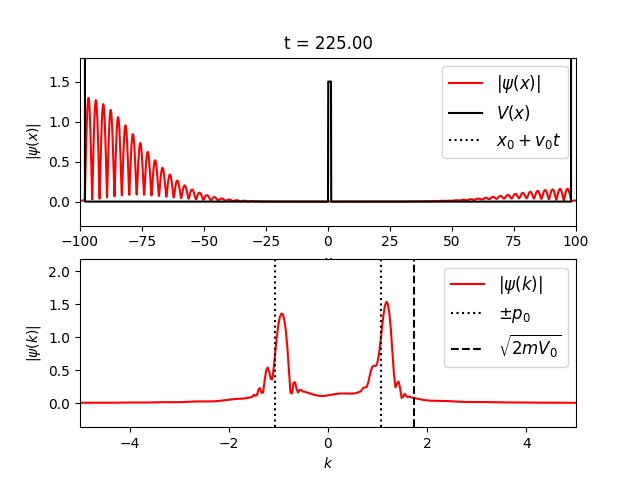
\includegraphics[width=\linewidth]{pics/P6.1.png}
    \end{minipage}%
    \begin{minipage}{0.5\textwidth}
        \centering
        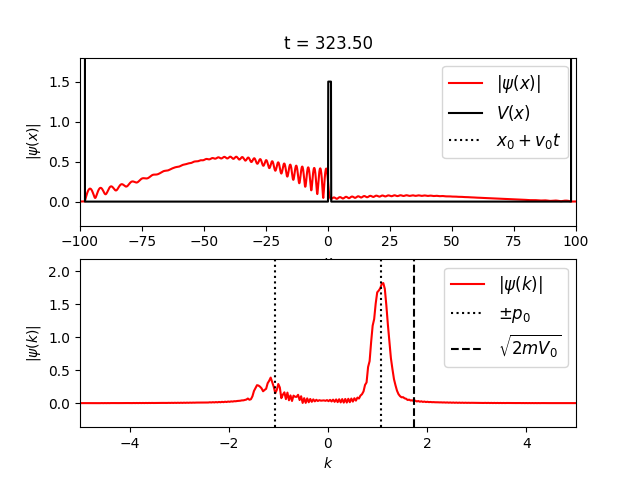
\includegraphics[width=\linewidth]{pics/P6.2.png}
    \end{minipage}
    \begin{minipage}{0.5\textwidth}
        \centering
        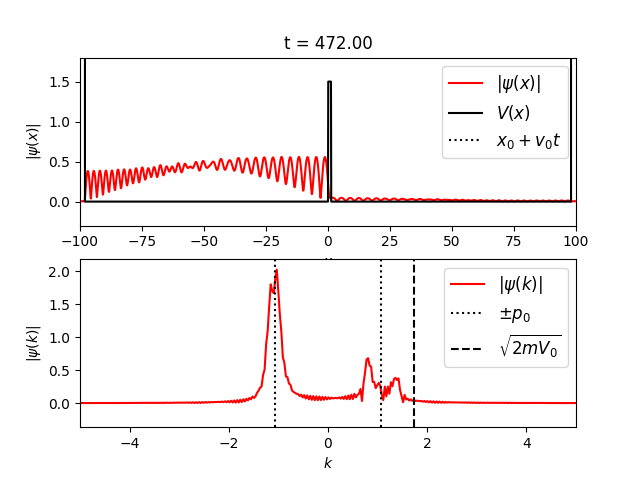
\includegraphics[width=\linewidth]{pics/P6.3.png}
    \end{minipage}%
    \begin{minipage}{0.5\textwidth}
        \centering
        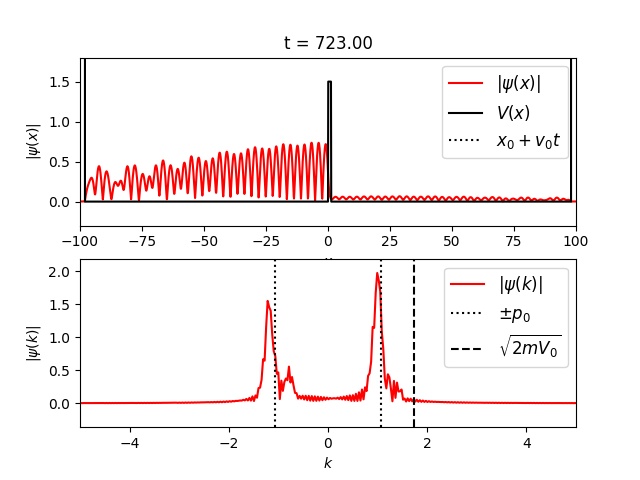
\includegraphics[width=\linewidth]{pics/P6.4.png}
    \end{minipage}
    \caption{不同状态下的快速傅里叶变换求薛定谔方程数值解结果}
\end{figure}
实验证明,快速傅里叶变换能较快且有效求解出薛定谔方程的数值解,具有非常好的应用效果。
\section{结论}
快速傅里叶变换可以高效地对微分方程进行数值求解,通过合理选择傅里叶级数的展开方式和截断技术,可以在保证精度的前提下极大地提高数值求解的效率。
\clearpage

\section{附录: 程序完整代码}
\lstset{
    numbers=left,
    language=Python,
    keywordstyle=\color{blue!100},
    commentstyle=\color{green!50!blue!50!},
    frame=shadowbox,%阴影
    escapeinside='',%英文分号输入中文
    xleftmargin=2em,xrightmargin=2em,aboveskip=1em,
    framexleftmargin=2em,
    extendedchars=false}

\begin{lstlisting}[aboveskip=0pt]
    import numpy as np
    from matplotlib import pyplot as pl
    from matplotlib import animation
    from scipy.fftpack import fft, ifft
    
    
    class Schrodinger(object):
        """
        Class which implements a numerical solution of the time-dependent
        Schrodinger equation for an arbitrary potential
        """
    
        def __init__(self, x, psi_x0, V_x,
                     k0=None, hbar=1, m=1, t0=0.0):
            """
            Parameters
            ----------
            x : array_like, float
                length-N array of evenly spaced spatial coordinates
            psi_x0 : array_like, complex
                length-N array of the initial wave function at time t0
            V_x : array_like, float
                 length-N array giving the potential at each x
            k0 : float
                the minimum value of k.  Note that, because of the workings of the
                fast fourier transform, the momentum wave-number will be defined
                in the range
                  k0 < k < 2*pi / dx
                where dx = x[1]-x[0].  If you expect nonzero momentum outside this
                range, you must modify the inputs accordingly.  If not specified,
                k0 will be calculated such that the range is [-k0,k0]
            hbar : float
                value of planck's constant (default = 1)
            m : float
                particle mass (default = 1)
            t0 : float
                initial tile (default = 0)
            """
            # Validation of array inputs
            self.x, psi_x0, self.V_x = map(np.asarray, (x, psi_x0, V_x))
            N = self.x.size
            assert self.x.shape == (N,)
            assert psi_x0.shape == (N,)
            assert self.V_x.shape == (N,)
    
            # Set internal parameters
            self.hbar = hbar
            self.m = m
            self.t = t0
            self.dt_ = None
            self.N = len(x)
            self.dx = self.x[1] - self.x[0]
            self.dk = 2 * np.pi / (self.N * self.dx)
    
            # set momentum scale
            if k0 == None:
                self.k0 = -0.5 * self.N * self.dk
            else:
                self.k0 = k0
            self.k = self.k0 + self.dk * np.arange(self.N)
    
            self.psi_x = psi_x0
            self.compute_k_from_x()
    
            # variables which hold steps in evolution of the
            self.x_evolve_half = None
            self.x_evolve = None
            self.k_evolve = None
    
            # attributes used for dynamic plotting
            self.psi_x_line = None
            self.psi_k_line = None
            self.V_x_line = None
    
        def _set_psi_x(self, psi_x):
            self.psi_mod_x = (psi_x * np.exp(-1j * self.k[0] * self.x)
                              * self.dx / np.sqrt(2 * np.pi))
    
        def _get_psi_x(self):
            return (self.psi_mod_x * np.exp(1j * self.k[0] * self.x)
                    * np.sqrt(2 * np.pi) / self.dx)
    
        def _set_psi_k(self, psi_k):
            self.psi_mod_k = psi_k * np.exp(1j * self.x[0]
                                            * self.dk * np.arange(self.N))
    
        def _get_psi_k(self):
            return self.psi_mod_k * np.exp(-1j * self.x[0] *
                                           self.dk * np.arange(self.N))
    
        def _get_dt(self):
            return self.dt_
    
        def _set_dt(self, dt):
            if dt != self.dt_:
                self.dt_ = dt
                self.x_evolve_half = np.exp(-0.5 * 1j * self.V_x
                                            / self.hbar * dt)
                self.x_evolve = self.x_evolve_half * self.x_evolve_half
                self.k_evolve = np.exp(-0.5 * 1j * self.hbar /
                                       self.m * (self.k * self.k) * dt)
    
        psi_x = property(_get_psi_x, _set_psi_x)
        psi_k = property(_get_psi_k, _set_psi_k)
        dt = property(_get_dt, _set_dt)
    
        def compute_k_from_x(self):
            self.psi_mod_k = fft(self.psi_mod_x)
    
        def compute_x_from_k(self):
            self.psi_mod_x = ifft(self.psi_mod_k)
    
        def time_step(self, dt, Nsteps=1):
            """
            Perform a series of time-steps via the time-dependent
            Schrodinger Equation.
    
            Parameters
            ----------
            dt : float
                the small time interval over which to integrate
            Nsteps : float, optional
                the number of intervals to compute.  The total change
                in time at the end of this method will be dt * Nsteps.
                default is N = 1
            """
            self.dt = dt
    
            if Nsteps > 0:
                self.psi_mod_x *= self.x_evolve_half
    
            for i in range(Nsteps - 1):
                self.compute_k_from_x()
                self.psi_mod_k *= self.k_evolve
                self.compute_x_from_k()
                self.psi_mod_x *= self.x_evolve
    
            self.compute_k_from_x()
            self.psi_mod_k *= self.k_evolve
    
            self.compute_x_from_k()
            self.psi_mod_x *= self.x_evolve_half
    
            self.compute_k_from_x()
    
            self.t += dt * Nsteps
    
    
    ######################################################################
    # Helper functions for gaussian wave-packets
    
    def gauss_x(x, a, x0, k0):
        """
        a gaussian wave packet of width a, centered at x0, with momentum k0
        """
        return ((a * np.sqrt(np.pi)) ** (-0.5)
                * np.exp(-0.5 * ((x - x0) * 1. / a) ** 2 + 1j * x * k0))
    
    
    def gauss_k(k, a, x0, k0):
        """
        analytical fourier transform of gauss_x(x), above
        """
        return ((a / np.sqrt(np.pi))**0.5
                * np.exp(-0.5 * (a * (k - k0)) ** 2 - 1j * (k - k0) * x0))
    
    
    ######################################################################
    # Utility functions for running the animation
    
    def theta(x):
        """
        theta function :
          returns 0 if x<=0, and 1 if x>0
        """
        x = np.asarray(x)
        y = np.zeros(x.shape)
        y[x > 0] = 1.0
        return y
    
    
    def square_barrier(x, width, height):
        return height * (theta(x) - theta(x - width))
    
    ######################################################################
    # Create the animation
    
    
    # specify time steps and duration
    dt = 0.01
    N_steps = 50
    t_max = 120
    frames = int(t_max / float(N_steps * dt))
    
    # specify constants
    hbar = 1.0   # planck's constant
    m = 1.9      # particle mass
    
    # specify range in x coordinate
    N = 2 ** 11
    dx = 0.1
    x = dx * (np.arange(N) - 0.5 * N)
    
    # specify potential
    V0 = 1.5
    L = hbar / np.sqrt(2 * m * V0)
    a = 3 * L
    x0 = -60 * L
    V_x = square_barrier(x, a, V0)
    V_x[x < -98] = 1E6
    V_x[x > 98] = 1E6
    
    # specify initial momentum and quantities derived from it
    p0 = np.sqrt(2 * m * 0.2 * V0)
    dp2 = p0 * p0 * 1./80
    d = hbar / np.sqrt(2 * dp2)
    
    k0 = p0 / hbar
    v0 = p0 / m
    psi_x0 = gauss_x(x, d, x0, k0)
    
    # define the Schrodinger object which performs the calculations
    S = Schrodinger(x=x,
                    psi_x0=psi_x0,
                    V_x=V_x,
                    hbar=hbar,
                    m=m,
                    k0=-28)
    
    ######################################################################
    # Set up plot
    fig = pl.figure()
    
    # plotting limits
    xlim = (-100, 100)
    klim = (-5, 5)
    
    # top axes show the x-space data
    ymin = 0
    ymax = V0
    ax1 = fig.add_subplot(211, xlim=xlim,
                          ylim=(ymin - 0.2 * (ymax - ymin),
                                ymax + 0.2 * (ymax - ymin)))
    psi_x_line, = ax1.plot([], [], c='r', label=r'$|\psi(x)|$')
    V_x_line, = ax1.plot([], [], c='k', label=r'$V(x)$')
    center_line = ax1.axvline(0, c='k', ls=':',
                              label=r"$x_0 + v_0t$")
    
    title = ax1.set_title("")
    ax1.legend(prop=dict(size=12))
    ax1.set_xlabel('$x$')
    ax1.set_ylabel(r'$|\psi(x)|$')
    
    # bottom axes show the k-space data
    ymin = abs(S.psi_k).min()
    ymax = abs(S.psi_k).max()
    ax2 = fig.add_subplot(212, xlim=klim,
                          ylim=(ymin - 0.2 * (ymax - ymin),
                                ymax + 0.2 * (ymax - ymin)))
    psi_k_line, = ax2.plot([], [], c='r', label=r'$|\psi(k)|$')
    
    p0_line1 = ax2.axvline(-p0 / hbar, c='k', ls=':', label=r'$\pm p_0$')
    p0_line2 = ax2.axvline(p0 / hbar, c='k', ls=':')
    mV_line = ax2.axvline(np.sqrt(2 * V0) / hbar, c='k', ls='--',
                          label=r'$\sqrt{2mV_0}$')
    ax2.legend(prop=dict(size=12))
    ax2.set_xlabel('$k$')
    ax2.set_ylabel(r'$|\psi(k)|$')
    
    V_x_line.set_data(S.x, S.V_x)
    
    ######################################################################
    # Animate plot
    
    
    def init():
        psi_x_line.set_data([], [])
        V_x_line.set_data([], [])
        center_line.set_data([], [])
    
        psi_k_line.set_data([], [])
        title.set_text("")
        return (psi_x_line, V_x_line, center_line, psi_k_line, title)
    
    
    def animate(i):
        S.time_step(dt, N_steps)
        psi_x_line.set_data(S.x, 4 * abs(S.psi_x))
        V_x_line.set_data(S.x, S.V_x)
        center_line.set_data(2 * [x0 + S.t * p0 / m], [0, 1])
    
        psi_k_line.set_data(S.k, abs(S.psi_k))
        title.set_text("t = %.2f" % S.t)
        return (psi_x_line, V_x_line, center_line, psi_k_line, title)
    
    
    # call the animator.  blit=True means only re-draw the parts that have changed.
    anim = animation.FuncAnimation(fig, animate, init_func=init,
                                   frames=frames, interval=30, blit=True)
    
    
    # uncomment the following line to save the video in mp4 format.  This
    # requires either mencoder or ffmpeg to be installed on your system
    
    #anim.save('schrodinger_barrier.mp4', fps=15, extra_args=['-vcodec', 'libx264'])
    
    pl.show()
\end{lstlisting}

\clearpage


\bibliographystyle{unsrt}
\bibliography{Reference}
\end{document}